\chapter{实验及结果分析}
在本章节中,我们首先介绍了本文使用的数据集,然后描述了实验中采用的评价方法,紧接着给出了用于对比实验的若干基线系统,
同时设计了几组实验来评估本文提出的长短期兴趣模型的有效性,最后我们对实验结果进行了分析和总结。

\section{实验设定}
本文选取了两种真实的数据集,一种是美国明尼苏达大学GroupLens研究组采集的由MovieLens网站用户提供的电影评分数据,
另一种是2006年电影租赁网站Netflix举办的百万美金大奖赛中采用的评测数据集,下面分别介绍这两种数据集的详细情况。

\subsection{MovieLens数据集}
著名网站MovieLens\footnote{http://movielens.org}是一个非盈利性质的个性化电影推荐网站,
该网站通过用户显示设置和用户历史电影评分数据建立了定制化的用户兴趣画像,
帮助用户发现其可能喜欢观看的电影,用户界面如图\ref{fig:movielens}所示。

\begin{figure}[htbp]
\centering
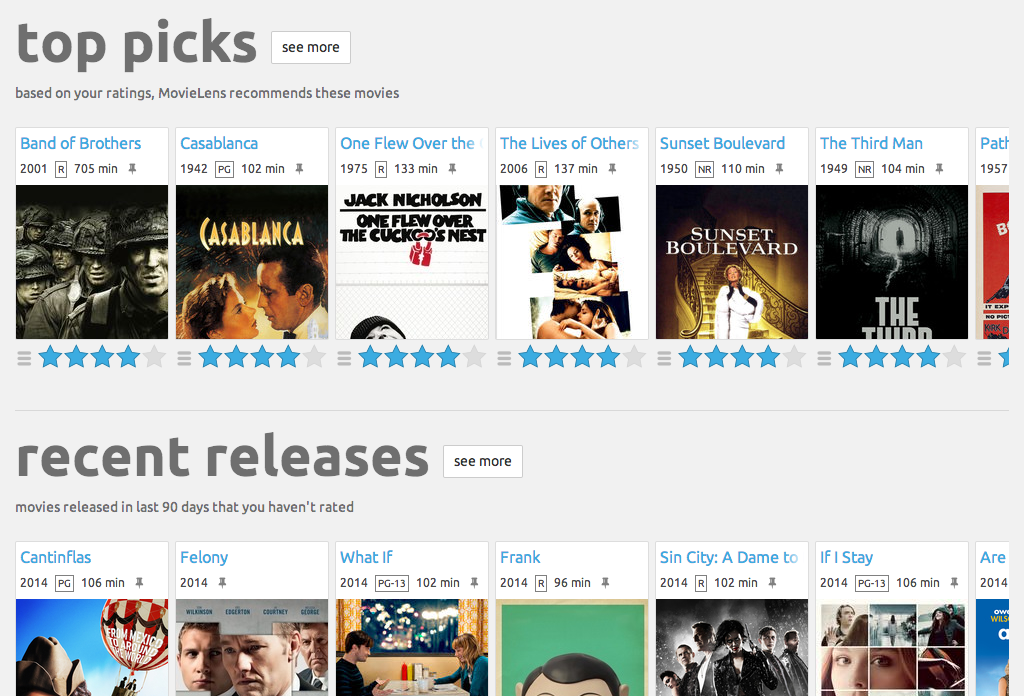
\includegraphics[scale=0.36]{images/movielens.png}
\caption{MovieLens网站上的电影推荐用户界面}
\label{fig:movielens}
\end{figure}

MovieLens网站由美国明尼苏达大学GroupLens研究组维护,常年以来,
GroupLens研究组致力于在MovieLens网站上收集用户电影评分数据,
并隐藏用户个人隐私信息,将其封装为公开的数据集贡献给推荐系统研究领域作为基准数据集,
用以帮助研究人员评测推荐算法的推荐性能。

MovieLens数据集包含若干子数据集,本文选取了其中的三个,按照评分数量的大小,
三个子数据集分别被命名为MovieLens-1M,MovieLens-10M和MovieLens-20M。

\begin{itemize}
\item \textbf{MovieLens-1M}数据集于2003年发布,其中包含$6,040$位用户,
$3,706$部电影以及$1,000,209$个评分数据,评分数据的取值范围是$1$分至$5$分,间隔为$1$分。
其中还提供了性别、年龄、职业和邮编等用户画像数据,标题、类别和发布年份等电影属性数据。
为了保证数据的有效性,每位用户至少拥有$20$个电影评分数据,整个数据集上的稀疏度为$95.53\%$。

\item \textbf{MovieLens-10M}数据集收集于2009年,其中包含$69,878$位用户,
$10,677$部电影以及$10,000,054$个评分数据,评分数据的取值范围是$0.5$分至$5$分,间隔为$0.5$分。
同时MovieLens-10M数据集还提供了$95,580$条标签数据,标签数据是推荐系统中重要的辅助数据,
基于标签的推荐系统也是一个重要的研究分支,
不少研究者\parencite{sigurbjornsson2008flickr,rendle2010pairwise,wang2015relational}致力于如何有效利用标签数据提升推荐效果。
不同于以往的数据集,为了保证用户的个人隐私权益,MovieLens-10M数据集不再提供用户画像数据,
每个用户只使用去敏的ID表示,不再有其他个人数据提供。
为了保证数据的有效性,每位用户至少拥有$20$个电影评分数据,整个数据集上的稀疏度为$98.66\%$。

\item \textbf{MovieLens-20M}数据集和MovieLens-10M数据集结构类似,其发布于2015年,
包含$138,493$位用户,$26,744$部电影,$465,564$条标签数据以及$20,000,263$个评分数据,
评分数据的取值范围是$0.5$分至$5$分,间隔为$0.5$分。MovieLens-20M数据集不提供用户画像数据,
但是也在之前数据集上做了创新,在提供电影属性信息的同时,该数据集额外提供了三个ID:
$movieId$、$imdbId$和$tmdbId$,分别对应本部电影在MovieLens网站、
ImDb网站\footnote{http://www.imdb.com}和TheMovieDb网站\footnote{https://www.themoviedb.org}
上的电影属性页,研究者可以自行制作爬虫前往相关页面爬取特定的属性信息,例如导演、演员、获奖信息等等。
\end{itemize}

\subsection{Netflix数据集}
Netflix数据集来源于著名电影租赁网站Netflix的数据库。
2006年,Netflix网站设立了百万美金大奖赛\footnote{http://www.netflixprize.com},
征集能够使其推荐系统性能上升$10\%$的推荐算法,
吸引了来自全球186个国家四万多个队伍参赛,经过近三年的较量,
冠军队伍BPC(BellKor's Pragmatic Chaos)提出的融合算法才达到了预定目标,
该赛事的最终排名结果如图\ref{fig:netflix}所示。

\begin{figure}[htbp]
\centering
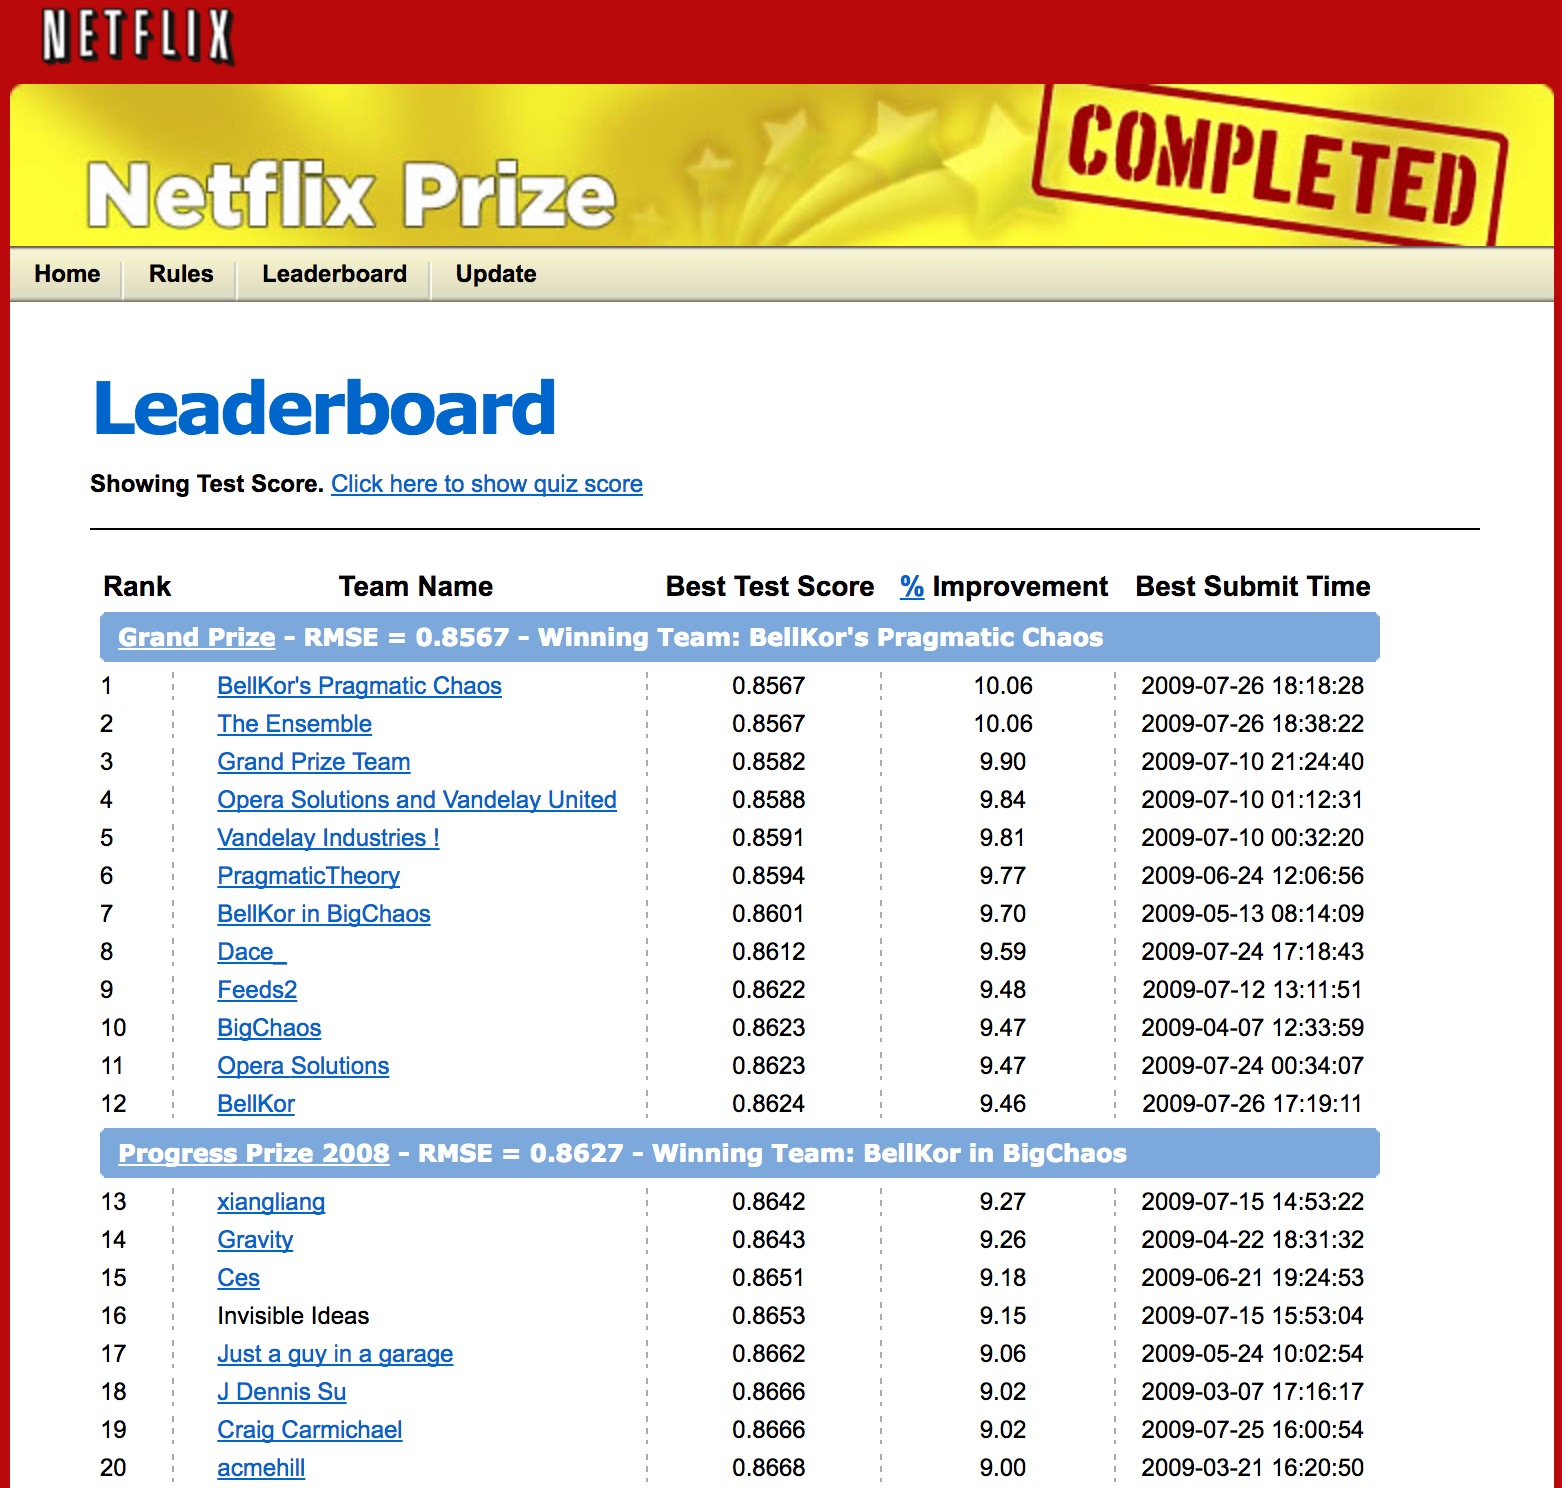
\includegraphics[scale=0.2]{images/netflix.jpeg}
\caption{Netflix百万美金大奖赛最终排名结果}
\label{fig:netflix}
\end{figure}

Netflix数据集发布于2006年,包含$480,189$位用户,$17,770$部电影以及$100,480,507$个评分数据,
评分数据的取值范围是$1$分至$5$分,间隔为$1$分。
Netflix数据集还提供了一些电影属性信息,包括电影标题和发布年份。
除此之外,为了方便参赛选手进行调参优化,该数据集还划分了相应的训练集、验证集和测试集。

\begin{table}[htbp]
    \centering
    \caption{MovieLens数据集和Netflix数据集的统计信息}
    \label{tab:statistics1}
        \begin{tabular}{|l|c|c|c|c|}
        \hline
        \textbf{Dataset} & \textbf{\#Users} & \textbf{\#Items} & \textbf{\#Ratings} & \textbf{Sparsity} \\
        \hline
        ML-1M   & 6,040   & 3,706  & 1,000,209   & 95.53\% \\
        ML-10M  & 69,878  & 10,677 & 10,000,054  & 98.66\% \\
        ML-20M  & 138,493 & 26,744 & 20,000,263  & 99.46\% \\
        Netflix & 480,189 & 17,770 & 100,480,507 & 98.82\% \\
        \hline
    \end{tabular}
\end{table}

\begin{table}[htbp]
    \centering
    \caption{MovieLens数据集和Netflix数据集的辅助信息}
    \label{tab:statistics2}
        \begin{tabular}{|l|c|c|c|}
        \hline
        \textbf{Dataset} & \textbf{UserInfo} & \textbf{ItemInfo} & \textbf{ItemTags} \\
        \hline
        ML-1M   & True  & True & False \\
        ML-10M  & False & True & True  \\
        ML-20M  & False & True & True  \\
        Netflix & False & True & False \\
        \hline
    \end{tabular}
\end{table}

表格\ref{tab:statistics1}和表格\ref{tab:statistics2}给出了所有四个数据集的统计信息和辅助信息,
包括用户数量,电影数量,评分数量、稀疏度,是否包含用户画像信息、是否包含电影属性信息和是否包含标签信息,
其中稀疏度的计算公式为:
\begin{equation}
\begin{split}
Sparsity = \frac{|Ratings|}{|Users| \cdot |Items|}
\end{split}
\end{equation}

\subsection{评价方法}
首先我们将数据集中的评分数据随机打乱,然后按照90\%和10\%的比例将其划分为训练集和测试集,
其中训练集$Train$用来训练本文提出的长短期兴趣模型和各类基线模型的最优参数,
测试集$Test$用来评价本文模型和各类基线模型的推荐性能。

由于本文中设计的推荐实验属于离线实验的一种,
同时为了与其他基线系统进行比较,
所以我们采用均方根误差$RMSE$和平均绝对误差$MAE$作为评价推荐效果的指标,
它们的计算公式如下:

\begin{equation}
RSME = \sqrt{ \frac{\sum_{i,j} I_{ij} (R_{ij} - \hat{R}_{ij})^2 } {|Test|} }
\end{equation}

\begin{equation}
MAE = \frac{\sum_{i,j} I_{ij} |R_{ij} - \hat{R}_{ij}|}{|Test|}
\end{equation}

其中$R_{ij}$代表用户$i$给电影$j$的真实评分数据,
$\hat{R}_{ij}$代表推荐算法预测用户$i$给电影$j$的估计评分数据,
$|Test|$是测试集中用户电影评分的总数量,
$I_{ij}$是一个二元矩阵,如果用户电影对$<i, j>$存在于测试集中,
则$I_{ij} = 1$,否则,$I_{ij} = 0$。

以上的实验步骤我们会重复$5$次,并取平均值作为最终的推荐得分,
这样做可以保证实验结果具有更好的说服力和更高的稳定性。
另外,对于测试集中出现的用户和电影,如果存在在训练集中不出现的情况,即冷启动问题(Cold-Start Problem),
推荐系统在这个场景下无法进行评分预测,我们会将其移出最后的评价结果。

\subsection{基线系统}
为了证明本文提出方法的有效性,我们实现了几类基线系统用于性能比较。

\subsubsection{基于规则的推荐算法}
基于规则的推荐算法是一种经验算法,由于其简便性在推荐系统研究初期备受关注。
从用户的角度来观察,性格宽容、习惯于评高分的用户在未来还更倾向于评高分,
持有批评态度、习惯打低分的用户在未来也更倾向于打低分;
从电影的角度来看,如果一部电影初始评分较高,那么未来评分也不会太差,
而如果初始评分较低,未来变成高分好片的概率也会很低。
所以本文首先实现了四种基于规则的推荐算法,分别描述如下:

(1)\textbf{GlobalMean}:对于测试集中的每一个用户电影对$<i, j>$,
我们使用训练集中的所有用户电影评分的平均值作为其预测评分。

(2)\textbf{UserMean}:对于测试集中的每一个用户电影对$<i, j>$,
我们使用训练集中的用户$i$的所有评分的平均值作为其预测评分。

(3)\textbf{ItemMean}:对于测试集中的每一个用户电影对$<i, j>$,
我们使用训练集中的电影$j$的所有评分的平均值作为其预测评分。

(4)\textbf{UserItemMean}:对于测试集中的每一个用户电影对$<i, j>$,
我们使用训练集中的用户$i$的评分均值和电影$j$的评分均值的折中作为其预测评分。

\subsubsection{基于矩阵分解的推荐算法}
由于在Netflix百万美金大奖赛中的突出表现,基于矩阵分解的推荐算法在近十年备受学术界和工业界的关注和投入。
以用户电影评分矩阵为例,矩阵分解就是将其分解为用户兴趣矩阵和电影兴趣矩阵,
在训练过程是使用已观察到的评分数据进行参数优化,
在预测的过程使用两个分解子矩阵相乘的结果作为预测缺失的评分数值,
然后基于预测评分数值以某种方式向用户进行推荐。
常见的矩阵分解方法有基本矩阵分解(Basic Matrix Factorization),
正则化矩阵分解(Regularized Matrix Factorization)
\parencite{koren2009matrix},
非负矩阵分解(Non-negative Matrix Factorization)
\parencite{lee2001algorithms},
概率矩阵分解(Probabilistic Matrix Factorization)
\parencite{salakhutdinov2007probabilistic}等。

LibMF是一个开源的矩阵分解工具包,由台湾国立大学的机器学习实验室开发并维护,
该实验室在机器学习领域享有盛名,近年来在多界KDD-Cup竞赛上取得了诸多优异的成绩。
LibMF在矩阵分解的并行化方面作出了良好的贡献,
针对随机梯度下降优化方法在并行计算中存在的锁问题(Locking Problem)和内存中断问题(Memory Discontinuity),
提出了一种矩阵分解的高效算法,根据计算节点的个数来划分评分矩阵块,并分配计算节点,可以在多核机器中并行计算,
在$17$亿评分数据集上只需不到$20$分钟即可收敛到一个较为合理的结果。
该工作\parencite{zhuang2013fast}发表在2013年的Recsys国际会议上,并获得了当年的最佳论文奖。

我们使用该开源工具包实现了一个基线模型,并将其标记为\textbf{LibMF}。

\subsubsection{基于因式分解机模型的推荐算法}
因式分解机(Factorization Machines, FM)是Rendle等人\parencite{rendle2010factorization}
在2010年提出的一种通用机器学习算法,通过特征工程模拟大多数分解模型,
可以对任意的实值向量进行预测。相比于其他机器学习算法,
因式分解机最大的特点是在高度稀疏数据场景下也拥有良好的学习能力,
同时线性的复杂度也保证了其在大型数据集的计算能力。

近几年,基于因式分解机模型的推荐算法成为推荐系统研究领域的一个研究热点,
在诸多推荐系统国际评测中都取得了优异的成绩。
目前,因式分解机的学习算法主要包括以下三种:
\begin{itemize}
\item 随机梯度下降法(Stochastic Gradient Descent, SGD)
\item 交替最小二乘法(Alternating Least-Squares, ALS)
\item 马尔科夫链蒙特卡罗法(Markov Chain Monte Carlo, MCMC)
\end{itemize}

LibFM \parencite{rendle2012factorization}是分解机的一个软件实现,
开源于Github网站上\footnote{https://github.com/srendle/libfm}。
我们使用该开源工具包上的三个学习算法实现了三个基线模型,
并将其标记为\textbf{LibFM-SGD}、\textbf{LibFM-ALS}和\textbf{LibFM-MCMC}。

\subsubsection{目前最优的推荐算法}
同样地,本文也提供了在学术界目前最优的推荐算法,主要包括两个工作。
第一个工作出自著名视频网站Hulu推荐团队Zheng等人\parencite{zheng2016neural},
该工作发表于机器学习领域国际顶级会议的ICML2016并受邀在会议上做口头报告。
这篇论文使用深度学习技术对推荐系统中的核心问题``协同滤波''进行建模,
并且在MovieLens-1M、MovieLens-10M和Netflix数据集上显著地提高了推荐性能,
达到了目前已知的最好结果。

因为Hulu的工作未涉及MovieLens-20M数据集,
所以本文又引用了Florian等人\parencite{strub2016hybrid}的工作。
他们改进了层叠去燥自动编码机(Stacked Denoising AutoEncoders)作为核心模型,
通过编码后再解码的方式,重构用户评分数据和电影评分数据,
利用瓶颈层学习出用户和电影的特征表示,在解码的过程中预测出未知的评分数据,
从而完成整个推荐过程,在MovieLens-20M数据集上取得目前已知的最好结果。

我们将两个工作的实验结果作为一个基线模型,标记为\textbf{SotA}(State-of-the-Art)。

\section{实验结果}
在本节中,我们报告实验结果来验证本文提出的长短期兴趣模型的有效性,本文中所有算法的超参数使用网格搜索(Grid Seach)的方法获得,
具体的设置设如下:

\begin{itemize}
\item
基于规则的基线系统无需设置超参数。
\item
基线系统\textbf{LibMF}中,我们设置隐因子的维度为$100$,优化算法的迭代次数为$1,000$。
\item
基线系统\textbf{LibFM-SGD}中,我们设置学习率为$0.01$,正则化参数为$(0,0,0.01)$,
二路因子的初始化标准差为$0.1$。
\item
基线系统\textbf{LibFM-ALS}中,我们设置正则化参数为$(0,0,10)$,
二路因子的初始化标准差为$0.1$。
\item
基线系统\textbf{LibFM-ALS}中,我们设置二路因子的初始化标准差为$0.1$。
\item
本文提出的多层感知器模型\textbf{UM}和\textbf{U-M}中,我们设置用户嵌入向量和电影嵌入向量的大小为$10$,
隐藏层的节点个数是输入层的节点个数的一半,训练过程中的学习率是$0.1$,用户和电影的正则化洗漱都为$0.01$。
\item
本文提出的长短期兴趣模型\textbf{LSIM}中,我们设置滑动窗口大小为$10$,隐因子的维度为$256$,
用户电影嵌入向量的维度为$100$。基于特征的协同过滤框架中,我们设置学习率$0.005$,
用户和电影的正则化系数都为$0.024$。
\item
目前最优的推荐系统中我们直接使用对应工作的实验结果,无需设置超参数。
\end{itemize}

\begin{table*}[htbp]
    \centering
    \caption{各个推荐算法在MovieLens数据集和Netflix数据集上的均方根误差表现}
    \label{tab:msre}
    \begin{tabular}{|l|c|c|c|c|}
        \hline
        \textbf{Algorithms} & \textbf{MovieLens-1M} & \textbf{MovieLens-10M} & \textbf{MovieLens-20M} & \textbf{Netflix} \\
        \hline
        GlobalMean   & 1.1181 $\pm$ 0.0008 & 1.0599 $\pm$ 0.0006 & 1.0518 $\pm$ 0.0003 & 1.0852 $\pm$ 0.0002 \\
        UserMean     & 1.0367 $\pm$ 0.0019 & 0.9775 $\pm$ 0.0005 & 0.9640 $\pm$ 0.0006 & 0.9986 $\pm$ 0.0001 \\
        ItemMean     & 0.9809 $\pm$ 0.0019 & 0.9432 $\pm$ 0.0008 & 0.9413 $\pm$ 0.0003 & 1.0112 $\pm$ 0.0002 \\
        UserItemMean & 0.9585 $\pm$ 0.0019 & 0.9125 $\pm$ 0.0007 & 0.9053 $\pm$ 0.0003 & 0.9639 $\pm$ 0.0002 \\
        \hline
        LibMF        & 0.8554 $\pm$ 0.0013 & 0.8090 $\pm$ 0.0004 & 0.8023 $\pm$ 0.0004 & 0.8630 $\pm$ 0.0002 \\
        \hline
        LibFM-SGD    & 0.8641 $\pm$ 0.0015 & 0.8022 $\pm$ 0.0013 & 0.7945 $\pm$ 0.0023 & 0.8485 $\pm$ 0.0014 \\
        LibFM-ALS    & 0.8453 $\pm$ 0.0015 & 0.7936 $\pm$ 0.0004 & 0.7860 $\pm$ 0.0004 & 0.8406 $\pm$ 0.0001 \\
        LibFM-MCMC   & 0.8460 $\pm$ 0.0011 & 0.7866 $\pm$ 0.0004 & 0.7787 $\pm$ 0.0005 & 0.8357 $\pm$ 0.0003 \\
        \hline
        UM           & 0.8630 $\pm$ 0.0016 & 0.8040 $\pm$ 0.0010 & 0.7970 $\pm$ 0.0008 & 0.8477 $\pm$ 0.0004 \\
        U-M          & 0.8566 $\pm$ 0.0012 & 0.7972 $\pm$ 0.0010 & 0.7864 $\pm$ 0.0003 & 0.8377 $\pm$ 0.0003 \\
        \hline
        LSIM         & \textbf{0.8355 $\pm$ 0.0014} & \textbf{0.7740 $\pm$ 0.0013} & \textbf{0.7656 $\pm$ 0.0019} & \textbf{0.8182 $\pm$ 0.0012} \\
        \hline
        SotA         & \textbf{0.8290} & \textbf{0.7710} & \textbf{0.7652} & \textbf{0.8030} \\
        \hline
    \end{tabular}
\end{table*}

表\ref{tab:msre}给出了本文提出的多层感知器模型、长短期兴趣模型以及各个基线系统方法在MovieLens数据集和Netflix数据集上的均方根误差表现。
我们将其分为$6$类,并在下面进行详细的分析。

\subsubsection{基于规则的推荐算法}
首先观察基于规则的四类推荐算法,\textbf{GlobalMean}使用全局均值作为预测得分,将所有的用户和电影一视同仁,没有区分能力,推荐效果最差。
\textbf{UserMean}和\textbf{ItemMean}分别单独考虑了用户偏好和电影偏好,推荐效果居中。而两者的优劣和数据集相关,
本文的实验中,\textbf{ItemMean}方法在MovieLens数据集上的效果较好,\textbf{UserMean}方法在Netflix数据集上的效果较好。
\textbf{UserItemMean}同时结合了用户偏好和电影偏好,效果是四者中最好的。本文中在结合用户偏好和电影偏好的方法中,
用户评分均值和电影评分均值各取一半,但是在具体的应用场景中两者的影响可能并不是等价的。
实际上还可以进一步将两者的系数作为训练参数由线性回归或者支持向量机训练得到,从而得到更好的推荐效果。

\subsubsection{基于矩阵分解的推荐算法}
紧接着观察基于矩阵分解的推荐算法,\textbf{LibMF}的整体效果比基于规则的推荐算法平均高出了$0.1$的得分,
但是却低于其他的基线系统(除了在MovieLens-1M数据集上效果比LibFM-SGD好之外)。
主要原因在于\textbf{LibMF}是一个优化模型,核心贡献在于加快矩阵分解的并行计算能力,
并没有过多地去优化原始的矩阵分解本身算法。事实上,在本文中的实验中,\textbf{LibMF}的训练时间
是除了基于规则外的算法中最短的。

\subsubsection{基于因式分解机的推荐算法}
然后观察基于因式分解机模型的推荐算法,里面包含三种学习算法。其中在数据集MovieLens-1M和Netflix上,\textbf{LibFM-ALS}的推荐性较好,
在数据集MovieLens-10M和MovieLens-20M上,\textbf{LibFM-MCMC}的表现更佳,具体到数据上来说,两者之间的差距是微乎其微的。
而\textbf{LibFM-SGD}在所有数据集上都是三者之中表现最差的。相比于\textbf{LibMF},基于因式分解机模型的推荐算法整体大概提升了$0.02$的推荐性能。

\subsubsection{基于多层感知器的推荐算法}
多层感知器模型主要包含两个模型\textbf{UM}和\textbf{U-M}。对于\textbf{UM}模型而言,它的整体实验结果和\textbf{LibMF}十分类似,
但是一个有趣的现象是,随着数据集大小的增加,\textbf{UM}模型的推荐性能从开始的低于\textbf{LibMF},到最后的反超,而且数据集越大两者的差距越大,
这充分体现了深度学习对数据量的依赖关系,只有保证提供足够的训练数据,深度学习才能发挥稳定且高效的实验性能。
对于\textbf{U-M}模型而言,我们主要将其和\textbf{UM}模型进行对比,整体的性能趋势上,\textbf{U-M}模型和\textbf{UM}模型十分类似,
都是随着数据量的增加推荐性能越来越好。但同时\textbf{U-M}模型在所有数据集上,都保持这比\textbf{UM}模型略高的推荐效果,
这也表明了本文提出的将用户嵌入表示和电影嵌入表示的差值作为额外输入的观点的有效性。

\subsubsection{基于长短期兴趣的推荐算法}
最后观察表中的倒数第二行,也就是本文提出的长短期兴趣模型的实验结果。在所有数据集上,\textbf{LSIM}的实验效果均高于其他所有基线系统,
推荐效果提升比例在$0.01$左右,这说明了长短期兴趣模型的有效性,利用用户的短期兴趣偏好确实有助于提升最终的预测结果。而且随着数据集的规格越大,
从MovieLens-1M到MovieLens-10M,再到MovieLens-20M和Netflix,长短期兴趣模型提升的比例也在进一步增加,从$0.01$提升至$0.02$,
这个现象主要说明了随着数据量的增加,长短期兴趣模型可以更高地从数据中学习出较优的用户表示和电影表示,从而预测评分的效果也会得到提升。

\subsubsection{当前最优的推荐算法}
对比长短期兴趣模型和目前最优的推荐算法的结果,我们发现两者的结果虽然比较接近,但是还是有一些差距,特别是在Netflix数据集上。
虽然都是使用深度学习方法对推荐系统进行优化,但是Hulu推荐团队的使用的网络结构更加复杂和深度,而本文中使用的网络结构比较简单和浅层,
这也为我们在未来的工作提供了一个良好的研究方向,如何设计更好的深度网络结构表示用户物品关系。

\begin{table*}[htbp]
    \centering
    \caption{各个推荐算法在MovieLens数据集和Netflix数据集上的平均绝对误差表现}
    \label{tab:mae}
    \begin{tabular}{|l|c|c|c|c|}
        \hline
        \textbf{Algorithms} & \textbf{MovieLens-1M} & \textbf{MovieLens-10M} & \textbf{MovieLens-20M} & \textbf{Netflix} \\
        \hline
        GlobalMean   & 0.9350 $\pm$ 0.0011 & 0.8550 $\pm$ 0.0005 & 0.8407 $\pm$ 0.0004 & 0.9095 $\pm$ 0.0002 \\
        UserMean     & 0.8300 $\pm$ 0.0017 & 0.7681 $\pm$ 0.0005 & 0.7516 $\pm$ 0.0005 & 0.7980 $\pm$ 0.0001 \\
        ItemMean     & 0.7840 $\pm$ 0.0012 & 0.7376 $\pm$ 0.0006 & 0.7317 $\pm$ 0.0002 & 0.8110 $\pm$ 0.0002 \\
        UserItemMean & 0.7726 $\pm$ 0.0014 & 0.7188 $\pm$ 0.0005 & 0.7077 $\pm$ 0.0003 & 0.7810 $\pm$ 0.0001 \\
        \hline
        LibMF        & 0.6816 $\pm$ 0.0008 & 0.6311 $\pm$ 0.0003 & 0.6229 $\pm$ 0.0004 & 0.6822 $\pm$ 0.0002 \\
        \hline
        LibFM-SGD    & 0.6674 $\pm$ 0.0027 & 0.6127 $\pm$ 0.0034 & 0.6016 $\pm$ 0.0036 & 0.6517 $\pm$ 0.0046 \\
        LibFM-ALS    & 0.6609 $\pm$ 0.0010 & 0.6068 $\pm$ 0.0002 & 0.5971 $\pm$ 0.0003 & 0.6481 $\pm$ 0.0002 \\
        LibFM-MCMC   & 0.6661 $\pm$ 0.0008 & 0.6039 $\pm$ 0.0002 & 0.5941 $\pm$ 0.0005 & 0.6486 $\pm$ 0.0002 \\
        \hline
        UM           & 0.6730 $\pm$ 0.0011 & 0.6145 $\pm$ 0.0009 & 0.6059 $\pm$ 0.0006 & 0.6555 $\pm$ 0.0006 \\
        U-M          & 0.6673 $\pm$ 0.0011 & 0.6083 $\pm$ 0.0009 & 0.5966 $\pm$ 0.0005 & 0.6454 $\pm$ 0.0003 \\
        \hline
        LSIM         & \textbf{0.6539 $\pm$ 0.0010} & \textbf{0.5928 $\pm$ 0.0013} & \textbf{0.5837 $\pm$ 0.0018} & \textbf{0.6337 $\pm$ 0.0014} \\
        \hline
    \end{tabular}
\end{table*}

表\ref{tab:mae}给出了本文提出的长短期兴趣模型和各个基线系统方法在MovieLens数据集和Netflix数据集上的平均绝对误差表现,
因为当前最优的推荐算法中没有使用平均绝对误差的指标,所以该表中并不包含相应的内容。
整体上来看,平均绝对误差在数值上比均方根误差小了$0.15$,这也从侧面反映了
在评分预测任务中,均方根误差和平均绝对误差虽然比较相似,但是均方根误差由于平方项的存在,
对大误差更加敏感,对预测算法的评价也更为苛刻。

整体的推荐效果方面上,平均绝对误差指标呈现和均方根误差指标类似的分布特征,分为4个分队,基于规则的推荐算法效果最差,处于第四分队;
基于矩阵分解的推荐算法把整体实验效果提升了$0.1$左右,位于第三分队;基于因式分解机的推荐算法处于第二分队,把推荐性能有提升了$0.02$;
基于多层感知器的推荐算法的推荐效果,处于基于矩阵分解的推荐算法和基于因式分解机的推荐算法两者的中间;
长短期兴趣模型效果最好,在基于因式分解机的推荐算法的基础上又大约提升了$0.01$的预测准确。

\section{实验讨论}
本文实现的实验中有许多可以进行讨论的地方,因为本文的主旨是深度学习在推荐系统中的应用,所以主要针对深度学习方面的内容进行实验讨论,
主要包括嵌入向量大小和训练数据量对实验结果的影响两类。

\subsection{多层感知器中嵌入向量大小的影响}
多层感知器模型中,为了将用户信息和电影信息输入到多层感知器中,我们首先利用嵌入矩阵获取了对应的用户嵌入向量和电影嵌入向量,
并且在训练过程中通过误差反向传播算法对其进行迭代更新。嵌入向量的大小可以体现模型为用户和电影创建了多大的空间存储它们的信息,
嵌入向量大小越大,能够存储的信息量也就越多,但多层感知器的的节点也会成倍增加,训练时间会被大大延长。
为了验证嵌入向量大小对推荐效果的影响,我们在MovieLens-1M数据集上设计了一些实验。在保证其他实验参数保持不变的前提下,
我们分别使用不同的嵌入向量大小进行了相应的实验。

\begin{figure}[htbp]
    \centering
    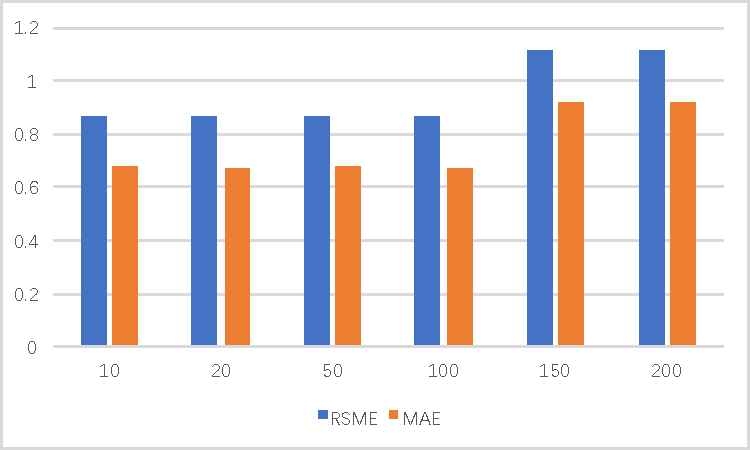
\includegraphics[scale=0.7]{images/UM.pdf}
    \caption{MovieLens-1M数据集上不同嵌入向量大小情况下均方根误差表现}
    \label{fig:um}
\end{figure}

\begin{figure}[htbp]
    \centering
    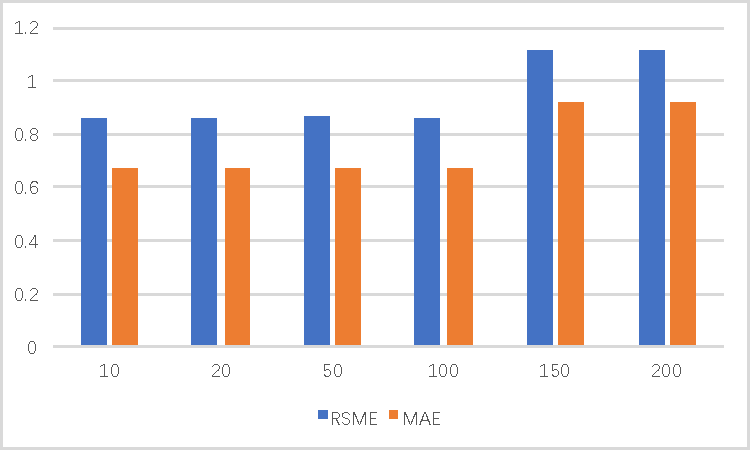
\includegraphics[scale=0.7]{images/U_M.pdf}
    \caption{MovieLens-1M数据集上不同嵌入向量大小情况下平均绝对误差表现}
    \label{fig:u_m}
\end{figure}

图\ref{fig:um}和图\ref{fig:u_m}分别给出了\textbf{UM}模型和\textbf{U-M}模型MovieLens-1M数据集上不同嵌入向量大小情况下
均方根误差表现和平均绝对误差表现,图表中的横坐标代表嵌入向量大小,分别从$10$,$20$增加到$150$和$200$,
纵坐标代表均方根误差和平均绝对误差的数值。两个图的整体趋势十分相似,令人惊讶的是,嵌入向量的大小对推荐效果的影响非常小,
在嵌入向量大小为$10$、$20$、$50$和$100$的情况下,均方根误差和平均绝对误差没有多大的变化,而是在小数点第三位上摆动,
这种现象的原因可能是数据集大小比较迷你,大小为$10$的嵌入向量已经能够足够存储用户信息和电影信息。
同时,在嵌入向量大小为$150$和$200$的情况下,均方根误差和平均绝对误差反而变大到和基于规则的全局均值推荐算法一样的水平线上,
我们观察具体的每一轮迭代更新中发现,均方根误差和平均绝对误差都没有下降的趋势,而是在初始值周围不断摆动,
这种现象的原因在于,嵌入向量大小过大导致多层感知器中的参数数量已经远远超过训练样本的数量,导致参数没有得到充分的学习,
即误差反向传播时没有办法对嵌入向量进行迭代更新。所以在具体的推荐场景中,我们应该充分实验得到一个较优的嵌入向量大小,
在保证推荐效果的同时,还可以节约推荐模型训练的时间。

\subsection{长短期兴趣模型的用户评分数量的影响}
在我们的长短期兴趣模型中,核心点在于利用用户的兴趣随着时间发生变化的特征,通过局部的评分数据,对用户的短期兴趣模型进行建模,
获得更好的用户特征表示和电影特征表示。如果一个用户在评分日志有较长的观影记录,那么他的长期兴趣分布和短期兴趣分布就可以细致地被长短期兴趣模型所提取;
但是如果一个用户的评分数据较为稀疏,无法体现用户的兴趣变化,长短期兴趣模型就无法充分学习用户的兴趣分布。
这种现象意味着长短期兴趣模型会在用户评分数据比较稠密的时候表现较优,但是在用户评分数据较为稀疏的场景下表现较差。

为了验证这样的猜想,我们在MovieLens-10M数据集上设计了一些实验。
首先我们将用户按照其评分数量由低到高进行排序,
然后均匀分到$5$个集合中,分别是$0\%$-$20\%$、$20\%$-$40\%$、$40\%$-$60\%$、$60\%$-$80\%$
和$80\%$-$100\%$。
其中$0\%$-$20\%$中包含评分数量最少的$20\%$的用户,$80\%$-$100\%$中包含评分数量最多的$20\%$的用户。
最后我们分别计算每个集合中在均方根误差和平均绝对误差上的表现。
整个实验的设定和上文类似,训练集和测试集的比例是$90\%$和$10\%$,
所有的实验重复$5$次,最终将平均值作为报告结果。

\begin{figure}[htbp]
    \centering
    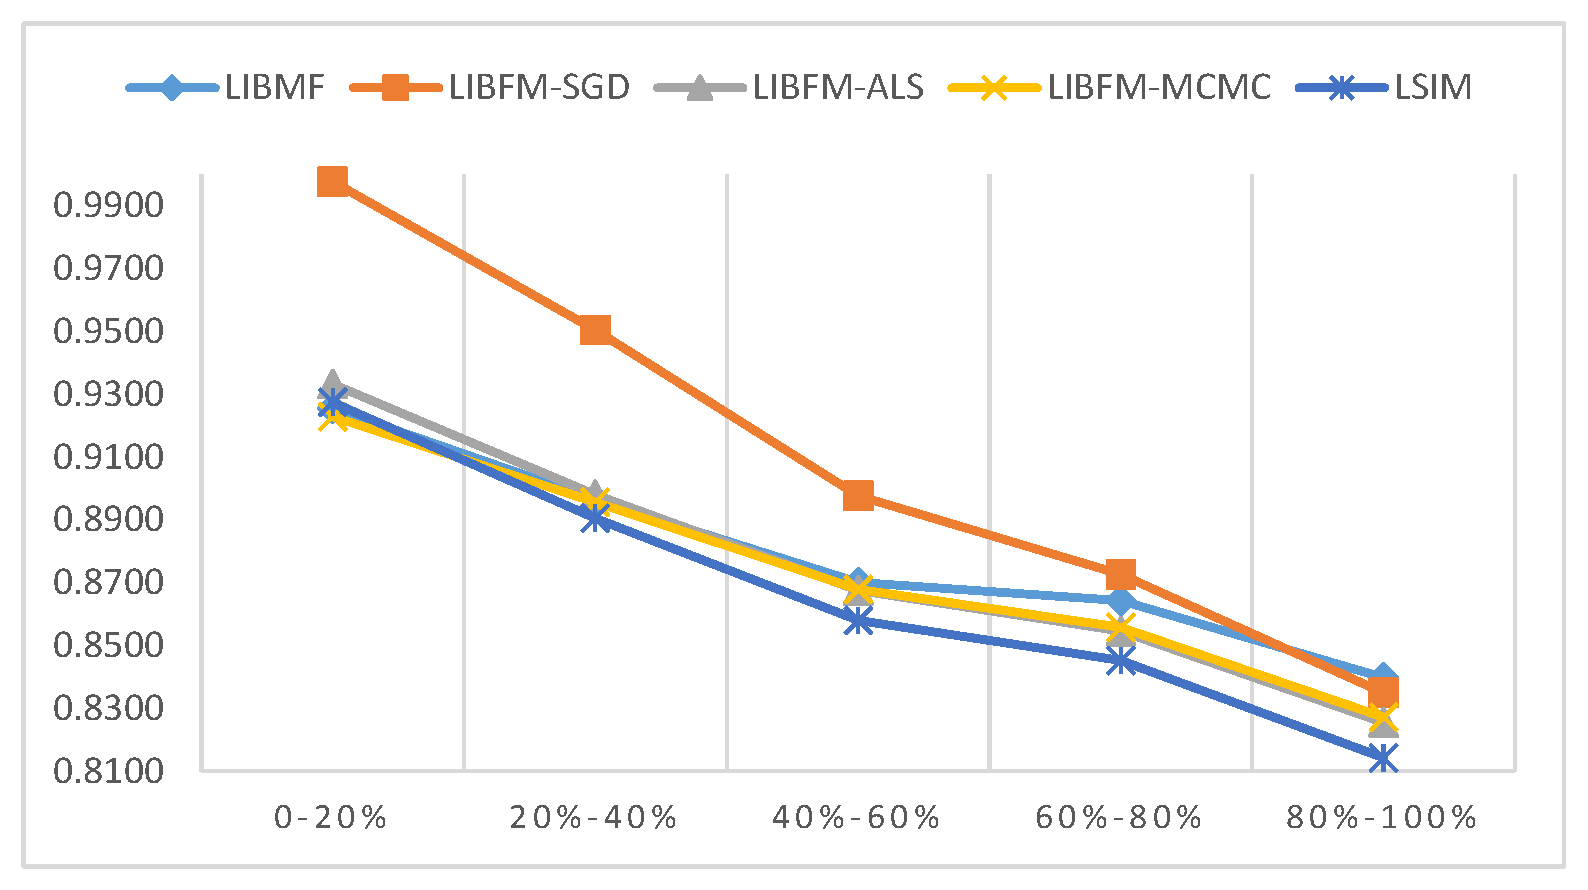
\includegraphics[scale=0.36]{images/rank_rmse.pdf}
    \caption{MovieLens-10M数据集评分数量由低到高的不同集合上的均方根误差表现}
    \label{fig:rank_rsme}
\end{figure}

\begin{figure}[htbp]
    \centering
    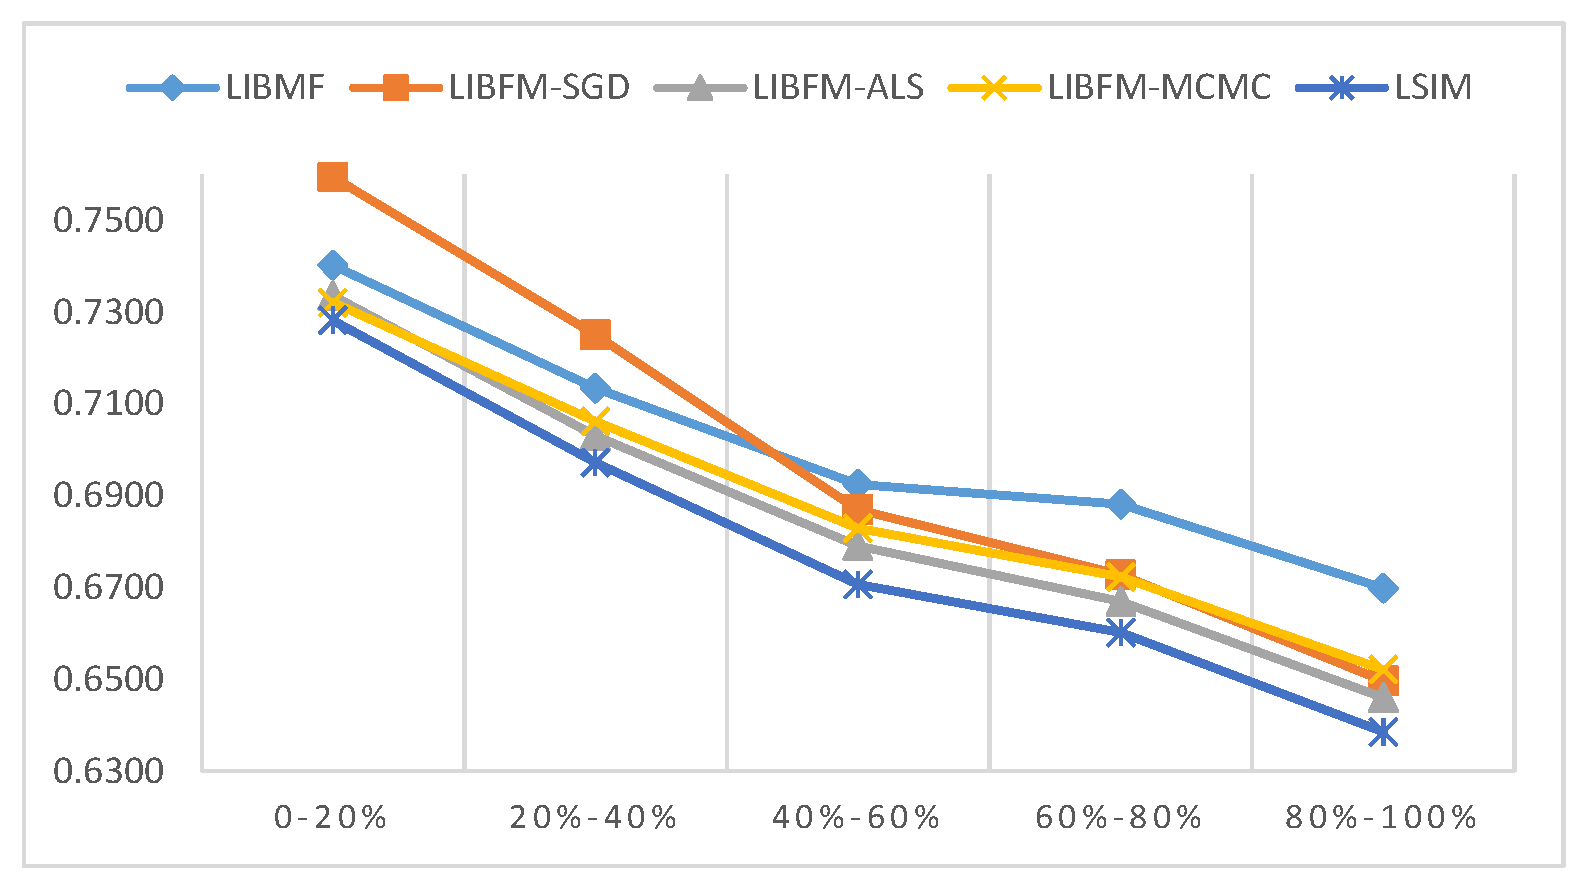
\includegraphics[scale=0.36]{images/rank_mae.pdf}
    \caption{MovieLens-10M数据集评分数量由低到高的不同集合上的平均绝对误差表现}
    \label{fig:rank_mae}
\end{figure}

图\ref{fig:rank_rsme}和图\ref{fig:rank_mae}分别给出了MovieLens-10M数据集评分数量由低到高的不同集合上的均方根误差表现和平均绝对误差表现,
从中可以明显看出,所有的推荐模型的推荐性能都随着用户评分数据的增加而提高,这个现象意味着用户和推荐系统的交互越多,推荐系统越能全方面地了解用户的偏好,
从而进行推荐更高的物品列表。同时本文提出的长短期兴趣模型在第一个集合上的均方根误差并不是很好,
$0.9275$的得分低于基于因式分解机的推荐模型\textbf{LibFM-MCMC},这主要是由于用户评分数量较少时,滑动窗口大小甚至会超过用户的评分数量,
会导致无法充分进行参数学习。但是随着评分数据的增多,长短期兴趣模型在之后的四个集合中推荐效果迅速提升,打败并逐渐拉大和其他基线模型的距离,
这个现象表明了长短期兴趣模型适用于一个生命周期较长的推荐系统场景,随着时间的推移,长短期兴趣模型可以进行越来越好的精准推荐。


